%% This is an example first chapter.  You should put chapter/appendix that you
%% write into a separate file, and add a line \include{yourfilename} to
%% main.tex, where `yourfilename.tex' is the name of the chapter/appendix file.
%% You can process specific files by typing their names in at the 
%% \files=
%% prompt when you run the file main.tex through LaTeX.

\singlespacing{

\chapter{Future Work}\label{chap:futureWork}

Future work revolves around hierarchical extensions of the current CAD/simulation model, experiments in computational design optimization, and development of a game around digital materials.

\section{Hierarchical Simulation}

\begin{figure}
  \includegraphics[width=\textwidth]{FunctionsParts.png}
  \caption{Three functional primitives decomposed as assemblies of elements.  The geometrical layout of elements within a functional primitive establish its mechanical and electronic properties.  Two sketches of a 1DOF Bending Flexure have different density, conductivity, and bending stiffnesses (top, middle).  Parallel plate construction of a capacitor determines the functional primitive's global capacitance (bottom).}
  \label{fig:FunctionsParts}
\end{figure}

The hierarchical construction of described in Chapter \ref{chapter:HierarchicalDesign} lends itself nicely to a hierarchical breakdown of CAD and simulation.  The bulk of this thesis explores CAD/simulation at the function-level, especially the decomposition of functional parts into functional primitives.  Current thoughts around the transition from assemblies of elements to functional primitives are depicted in Figures \ref{fig:FunctionsParts} and \ref{fig:HierarchicalSim}.\\

\begin{figure}
  \includegraphics[width=\textwidth]{HierarchicalSim.png}
  \caption{Schematic view of translation of an assembly of elements into parameters of a functional primitive.  Static simulation of assembly determines 15 stiffness constants, mass, and moment of inertia tensor.  Blue boxes indicate "holding points" for applied boundary conditions in static determination of multidimensional stiffness.}
  \label{fig:HierarchicalSim}
\end{figure}

Mechanical parameters describing a functional primitive are calculated from static simulations of assemblies of elements.  Boundary conditions applied to elements at each face of an assembly induce steady-state deformations.  15 sets of boundary conditions are used to calculate $F = kx$ and $T = k\theta$ for all 15 degrees of freedom (3 axial, 6 shear, 3 torsional, 3 bending).  For example, differences in composition between the two 1DOF bending flexures depicted in Figure \ref{fig:FunctionsParts} are expressed as differences stiffness constants at the functional primitive level of simulation (Figure \ref{fig:HierarchicalSim}).  In the case that these deformations are not linear over a range of applied forces, a constant $k$ is calculated to best fit the data.  Additionally, mass and inertia tensor are computed from assemblies of elements.\\

Electronic parameters may be determined as well.  Conductance between faces of a functional primitive are trivially calculated from assemblies of conducting and insulating elements.  Static capacitance and inductance may also computed using steady-state solutions to Finite Difference Time Domain (FDTD) simulations; previous work in DMDesign explored static electronic simulation (Figure \ref{fig:designAssemblyGUIWide}E).\\

Modules and complexes exhibit high-level behaviors that are abstracted from the low-level physics of the system.  The simulation of modules and complexes should reflect this increased abstraction.  I envision this type of simulation as a type of discretized, kinematic CA ruleset (somewhat like the work of William Stevens with CBlocks3D \ref{Stevens2009b}), though at this time it is unclear how to generate the governing ruleset from behaviors of assemblies of function-level parts.

\section{Computational Design Optimization}

Sets up nicely for computational design optimization

Constrained design space, due to the discretization of space and a limited set of potential parts types.

Low hanging fruit involves implementation of the element $\rightarrow$ functional primitive simulation and topological optimization of the patterning of elemental parts.


\section{"Fab the Game"}

An offshoot of the work described in this thesis is a collaboration with \href{http://elinemedia.com/}{E-Line Media} on a game.  Tentatively called "Fab the Game", it explores an aspirational future where digital materials are used to construct nearly everything.  

Players construct assemblies from functional primitives in an open-ended sandbox environment and in more directed challenges.  We envision a large component of gameplay revolves around constructing robots and using them to interact with and shape the surrounding environment.


Robots which are controlled in real time by players to compete in arena challenges, drawing inspiration from the competitions of \href{http://www.firstinspires.org/robotics/frc}{First Robotics}.


Players can dive into functional primitive definitions and alter the elemental composition to alter its function-level behavior.  Advanced gameplay involves designing new functional primitives from elemental part types to achieve behaviors beyond those provided by default.  We hope to encourage gameplay similar to what I've described exists around the Game of Life in Chapter \ref{chapter:HierarchicalDesign} and allow greater interaction with research at CBA.

Concept art by Eli Gershenfeld explores the look and feel of the game as well as potential gameplay scenarios (Figures \ref{fig:elibendy} through \ref{fig:elibridgefull}).

\begin{figure}
  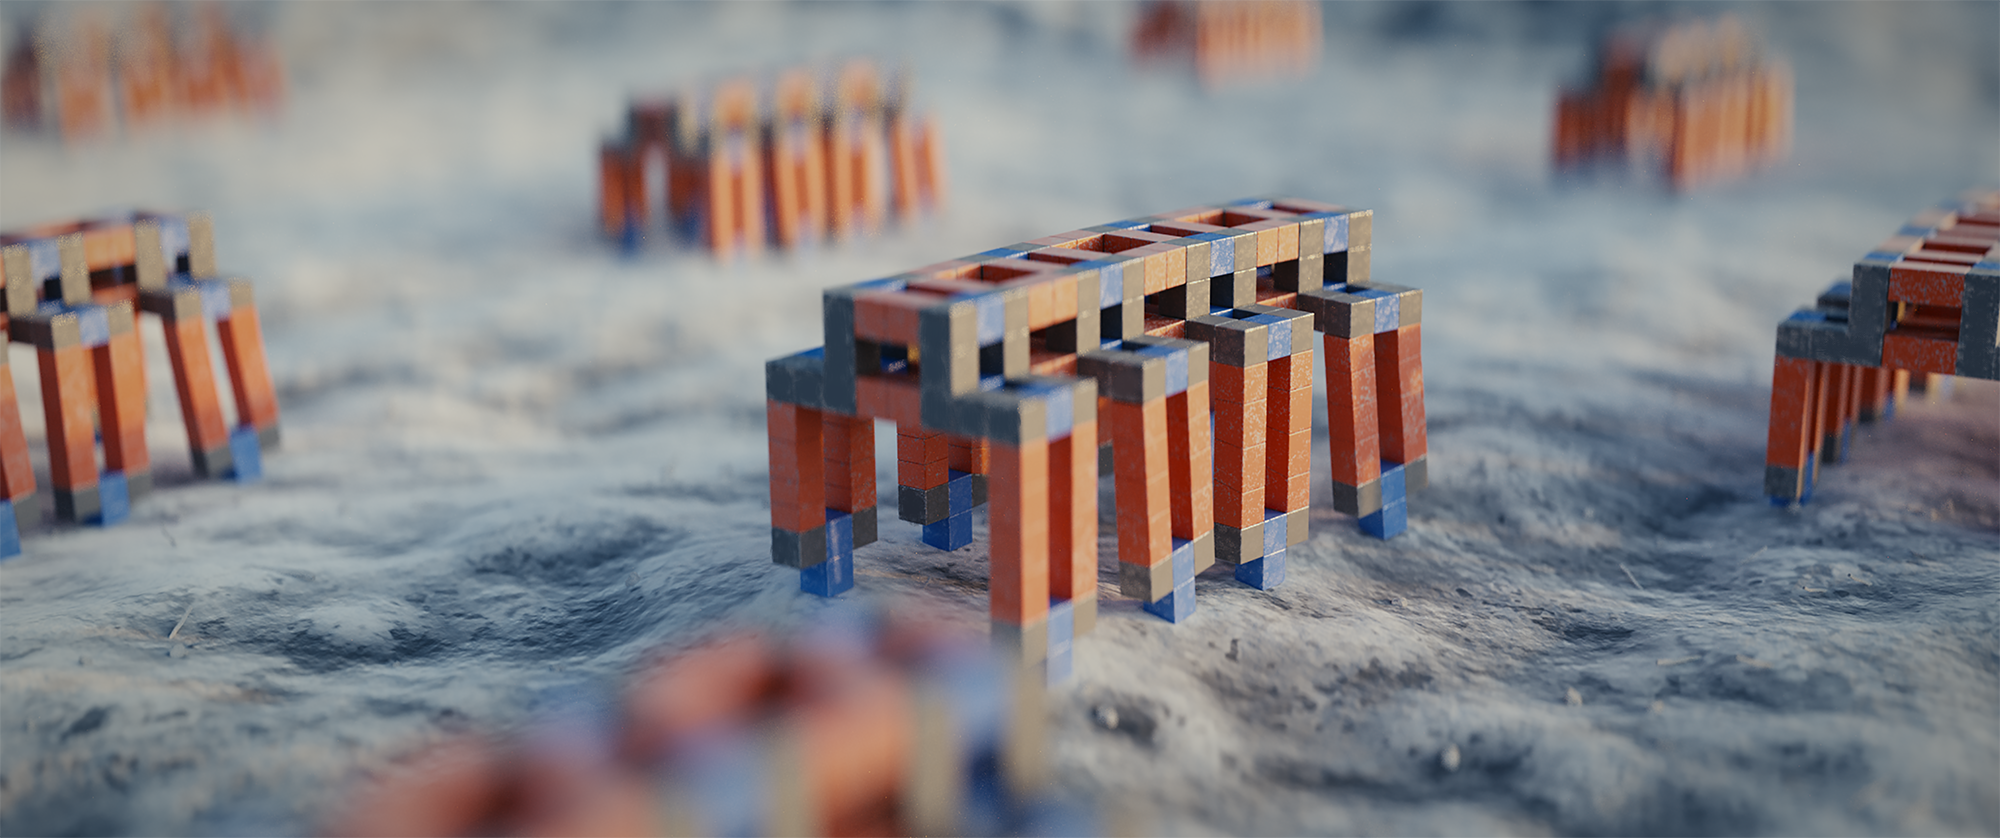
\includegraphics[width=\textwidth]{elibendy.png}
  \caption{A swarm of locomoting robots.  \textit{Image Credit: Eli Gershenfeld 2016}}
  \label{fig:elibendy}
\end{figure}

\begin{figure}
  \includegraphics[width=\textwidth]{eliassemblers.png}
  \caption{Assembler assembling an assembler.  \textit{Image Credit: Eli Gershenfeld 2016}}
  \label{fig:eliassemblers}
\end{figure}

\begin{figure}
  \includegraphics[width=\textwidth]{eliassembclose.png}
  \caption{Assembler "factory" feedstock.  \textit{Image Credit: Eli Gershenfeld 2016}}
  \label{fig:eliassembclose}
\end{figure}

\begin{figure}
  \includegraphics[width=\textwidth]{eliassembwide.png}
  \caption{Distributed "factory" automation. \textit{Image Credit: Eli Gershenfeld 2016}}
  \label{fig:eliassembwide}
\end{figure}

\begin{figure}
  \includegraphics[width=\textwidth]{elibridgeclose.png}
  \caption{"Living" macro-scale structure.  \textit{Image Credit: Eli Gershenfeld 2016}}
  \label{fig:elibridgeclose}
\end{figure}

\begin{figure}
  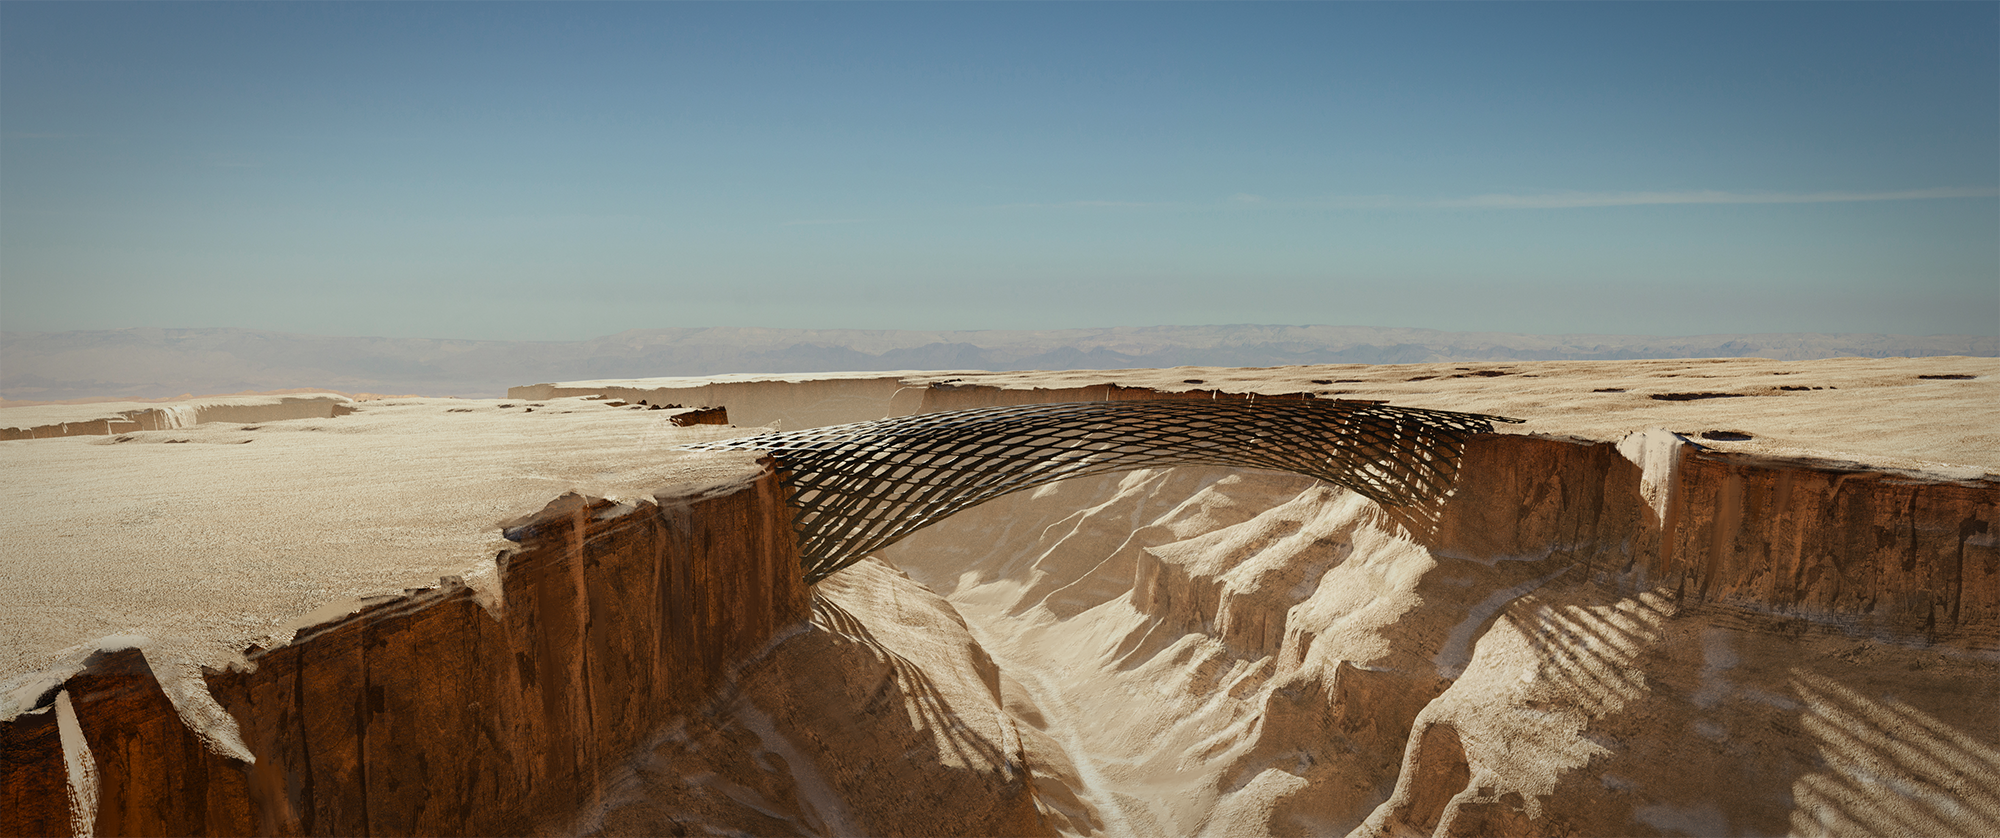
\includegraphics[width=\textwidth]{elibridgefull.png}
  \caption{Self-assembling bridge. \textit{Image Credit: Eli Gershenfeld 2016}}
  \label{fig:elibridgefull}
\end{figure}

